\section{Metodologia}

\subsection{Representação Multimodal de Entrada}
Para evitar ambiguidade entre variáveis simbólicas e nomes de sensores, representamos cada observação por um vetor de atributos multimodal ordenado:
\begin{equation}
\mathbf{x} = [x, y, \text{TEMP}, \text{COR}_{A}, \text{COR}_{V}] \in \mathbb{R}^{5},
\end{equation}
e um vetor-alvo de três saídas:
\begin{equation}
\mathbf{y} = [\text{pH}, \text{OD}, \text{TURB}] \in \mathbb{R}^{3}.
\end{equation}
Os atributos de entrada são normalizados antes da codificação em pulsos. Em seguida, aplicamos codificação por taxa (\textit{rate coding}), de modo que cada escalar normalizado é convertido em um trem de pulsos ao longo de $T$ passos de tempo, com probabilidade de disparo proporcional à sua magnitude. Isso produz uma representação temporal compatível com a dinâmica LIF subsequente, preservando a estrutura multimodal da amostra original.

\subsection{Arquitetura da SNN}
O modelo segue uma SNN \textit{feed-forward} com topologia $5 \rightarrow 64 \rightarrow 3$ e uma camada oculta de neurônios \textit{leaky integrate-and-fire} (LIF), como ilustrado na Fig.~\ref{fig:proposed_arch}. A atualização da membrana é
\begin{equation}
\mathbf{u}_{t+1} = \beta\,\mathbf{u}_{t} + \mathbf{W}\mathbf{s}_{t} - \theta\,\mathbf{z}_{t},
\end{equation}
onde $\beta$ é o decaimento da membrana, $\theta$ é o limiar de disparo e $\mathbf{z}_t$ são os pulsos emitidos. A predição de saída é calculada por agregação temporal ao longo dos passos.

\begin{figure}[!htbp]
\centering
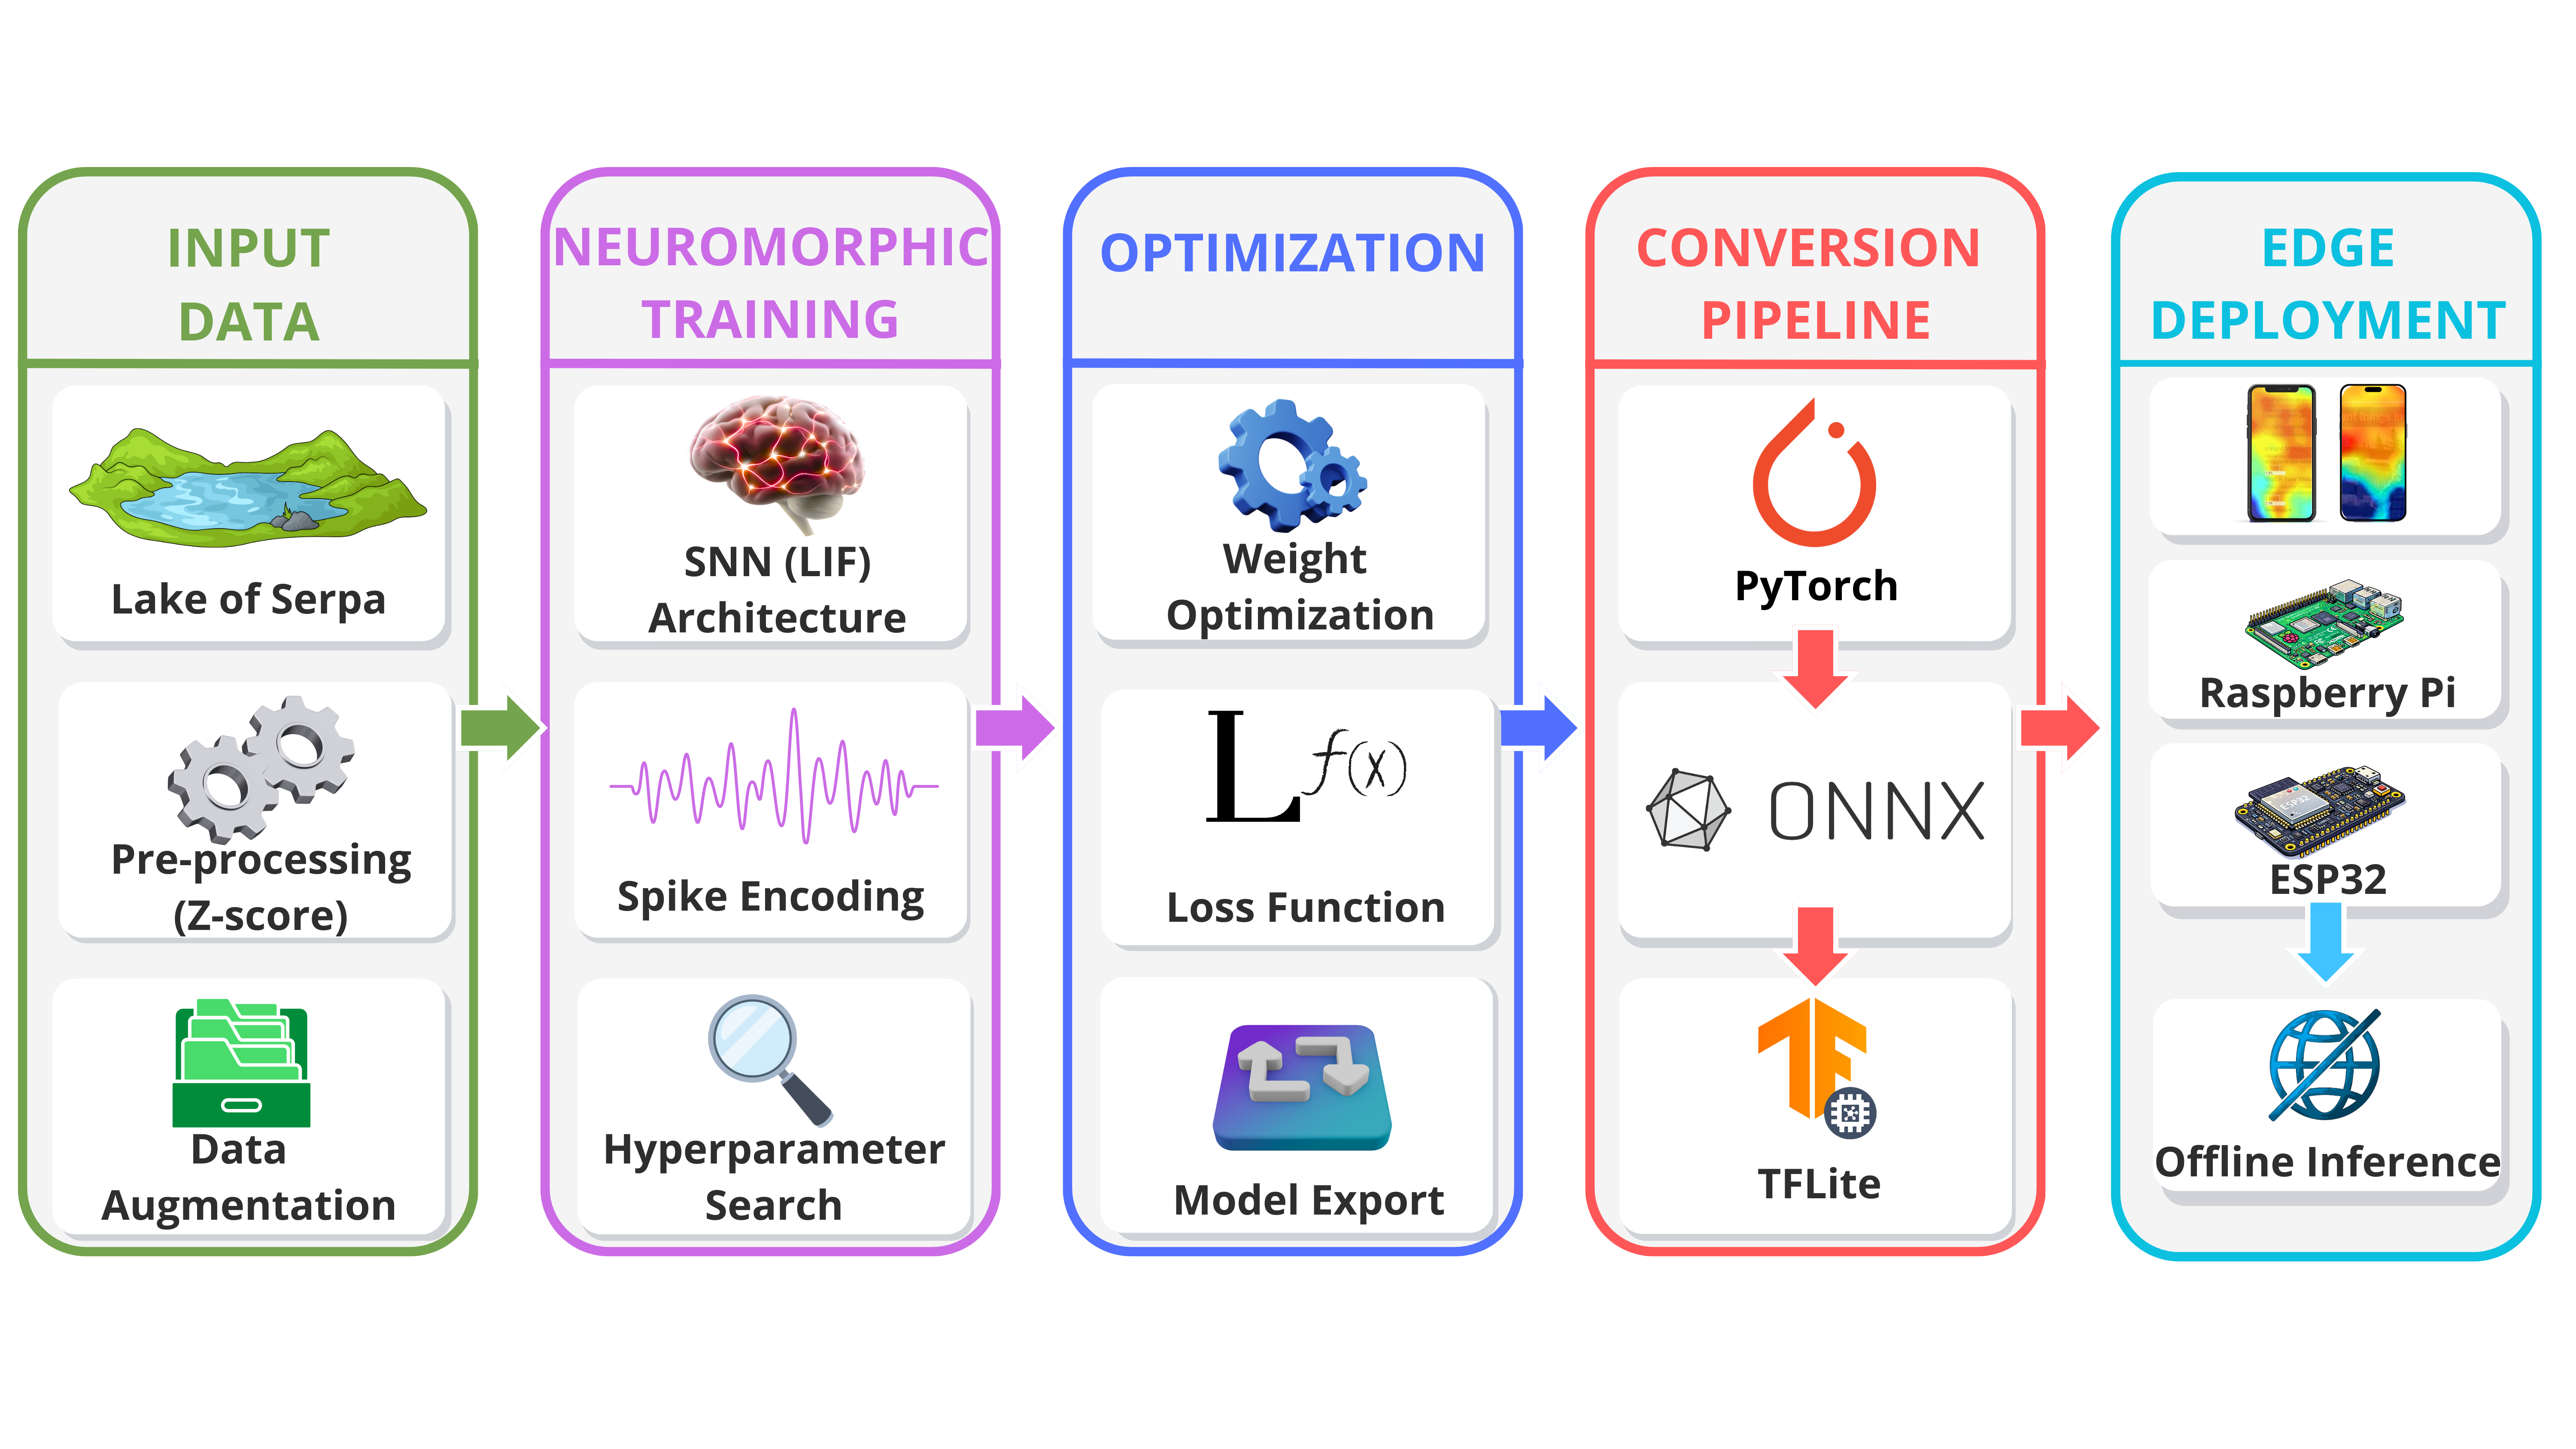
\includegraphics[width=0.58\linewidth]{Arquitetura.png}
\caption{Arquitetura SNN multimodal proposta para inferência offline na borda.}
\label{fig:proposed_arch}
\end{figure}

A Figura~\ref{fig:proposed_arch} apresenta o fluxo completo de ponta a ponta: preparação dos dados de campo (normalização e aumento controlado), treinamento neuromórfico com neurônios LIF e busca de hiperparâmetros, otimização e exportação do modelo pelo caminho de interoperabilidade PyTorch$\rightarrow$ONNX$\rightarrow$TFLite, e implantação offline na borda em Android, Raspberry Pi e ESP32.

\subsection{Protocolo de Treinamento}
O treinamento usou o otimizador Adam e perda MSE ponderada com parada antecipada. Os hiperparâmetros foram selecionados por busca em grade sobre tamanho da camada oculta, taxa de aprendizado, passos temporais $T$, limiar e fator de decaimento. \rev{O espaço de busca completo foi: tamanho da camada oculta $\in \{32, 64, 96\}$, $T \in \{10, 15, 25\}$, taxa de aprendizado \mbox{$\in \{0,0005;\, 0,001;\, 0,002\}$}, decaimento \mbox{$\beta \in \{0,90;\, 0,95\}$}, limiar \mbox{$\theta \in \{0,8;\, 1,0\}$} e ruído de aumento \mbox{$\sigma \in \{0,01;\, 0,02;\, 0,03\}$}, totalizando 324 configurações avaliadas pela perda de validação. A configuração selecionada foi: camada oculta 64, $T=15$, taxa de aprendizado \mbox{$0,002$}, \mbox{$\beta=0,95$}, \mbox{$\theta=0,8$} e \mbox{$\sigma=0,01$}.} A avaliação usou sementes aleatórias repetidas e métricas macro (MAE, RMSE e $R^2$) sobre os três alvos. \rev{As dez execuções independentes com sementes distintas implementam validação por subamostragem aleatória repetida, que aproxima o comportamento da validação cruzada neste regime de poucos dados; um protocolo k-fold completo está planejado para o conjunto de dados ampliado em campanhas futuras.}

\subsection{Sensibilidade aos Hiperparâmetros}
\rev{Os resultados da grade também fornecem uma análise de sensibilidade dos parâmetros LIF e da codificação temporal. Calculando a média marginal da perda de validação sobre as 324 configurações, a taxa de aprendizado teve o efeito mais forte (perda média de 0,826 em 0,0005 vs.~0,694 em 0,002). O limiar LIF mostrou preferência consistente por \mbox{$\theta=0,8$} em relação a \mbox{$\theta=1,0$} (0,747 vs.~0,769), enquanto o fator de decaimento teve influência menor (0,754 em \mbox{$\beta=0,90$} vs.~0,762 em \mbox{$\beta=0,95$}). O parâmetro temporal $T$ teve efeito fraco na acurácia (perda média de 0,766; 0,760 e 0,748 para \mbox{$T=10, 15, 25$}), mas o custo de inferência cresce aproximadamente de forma linear com $T$, já que cada passo adicional implica mais uma propagação direta de pulsos. Portanto, nesta tarefa, $T$ é primariamente um controle de energia--latência, e não de acurácia, e $T=15$ foi mantido como ponto de operação equilibrado.}

Como mostra a Fig.~\ref{fig:loss_curve_method}, as perdas de treinamento e validação diminuem rapidamente nas épocas iniciais e convergem para um platô estável com divergência limitada, indicando otimização consistente sem sobreajuste forte e apoiando o uso de parada antecipada neste regime de poucos dados.

\begin{figure}[!htbp]
\centering
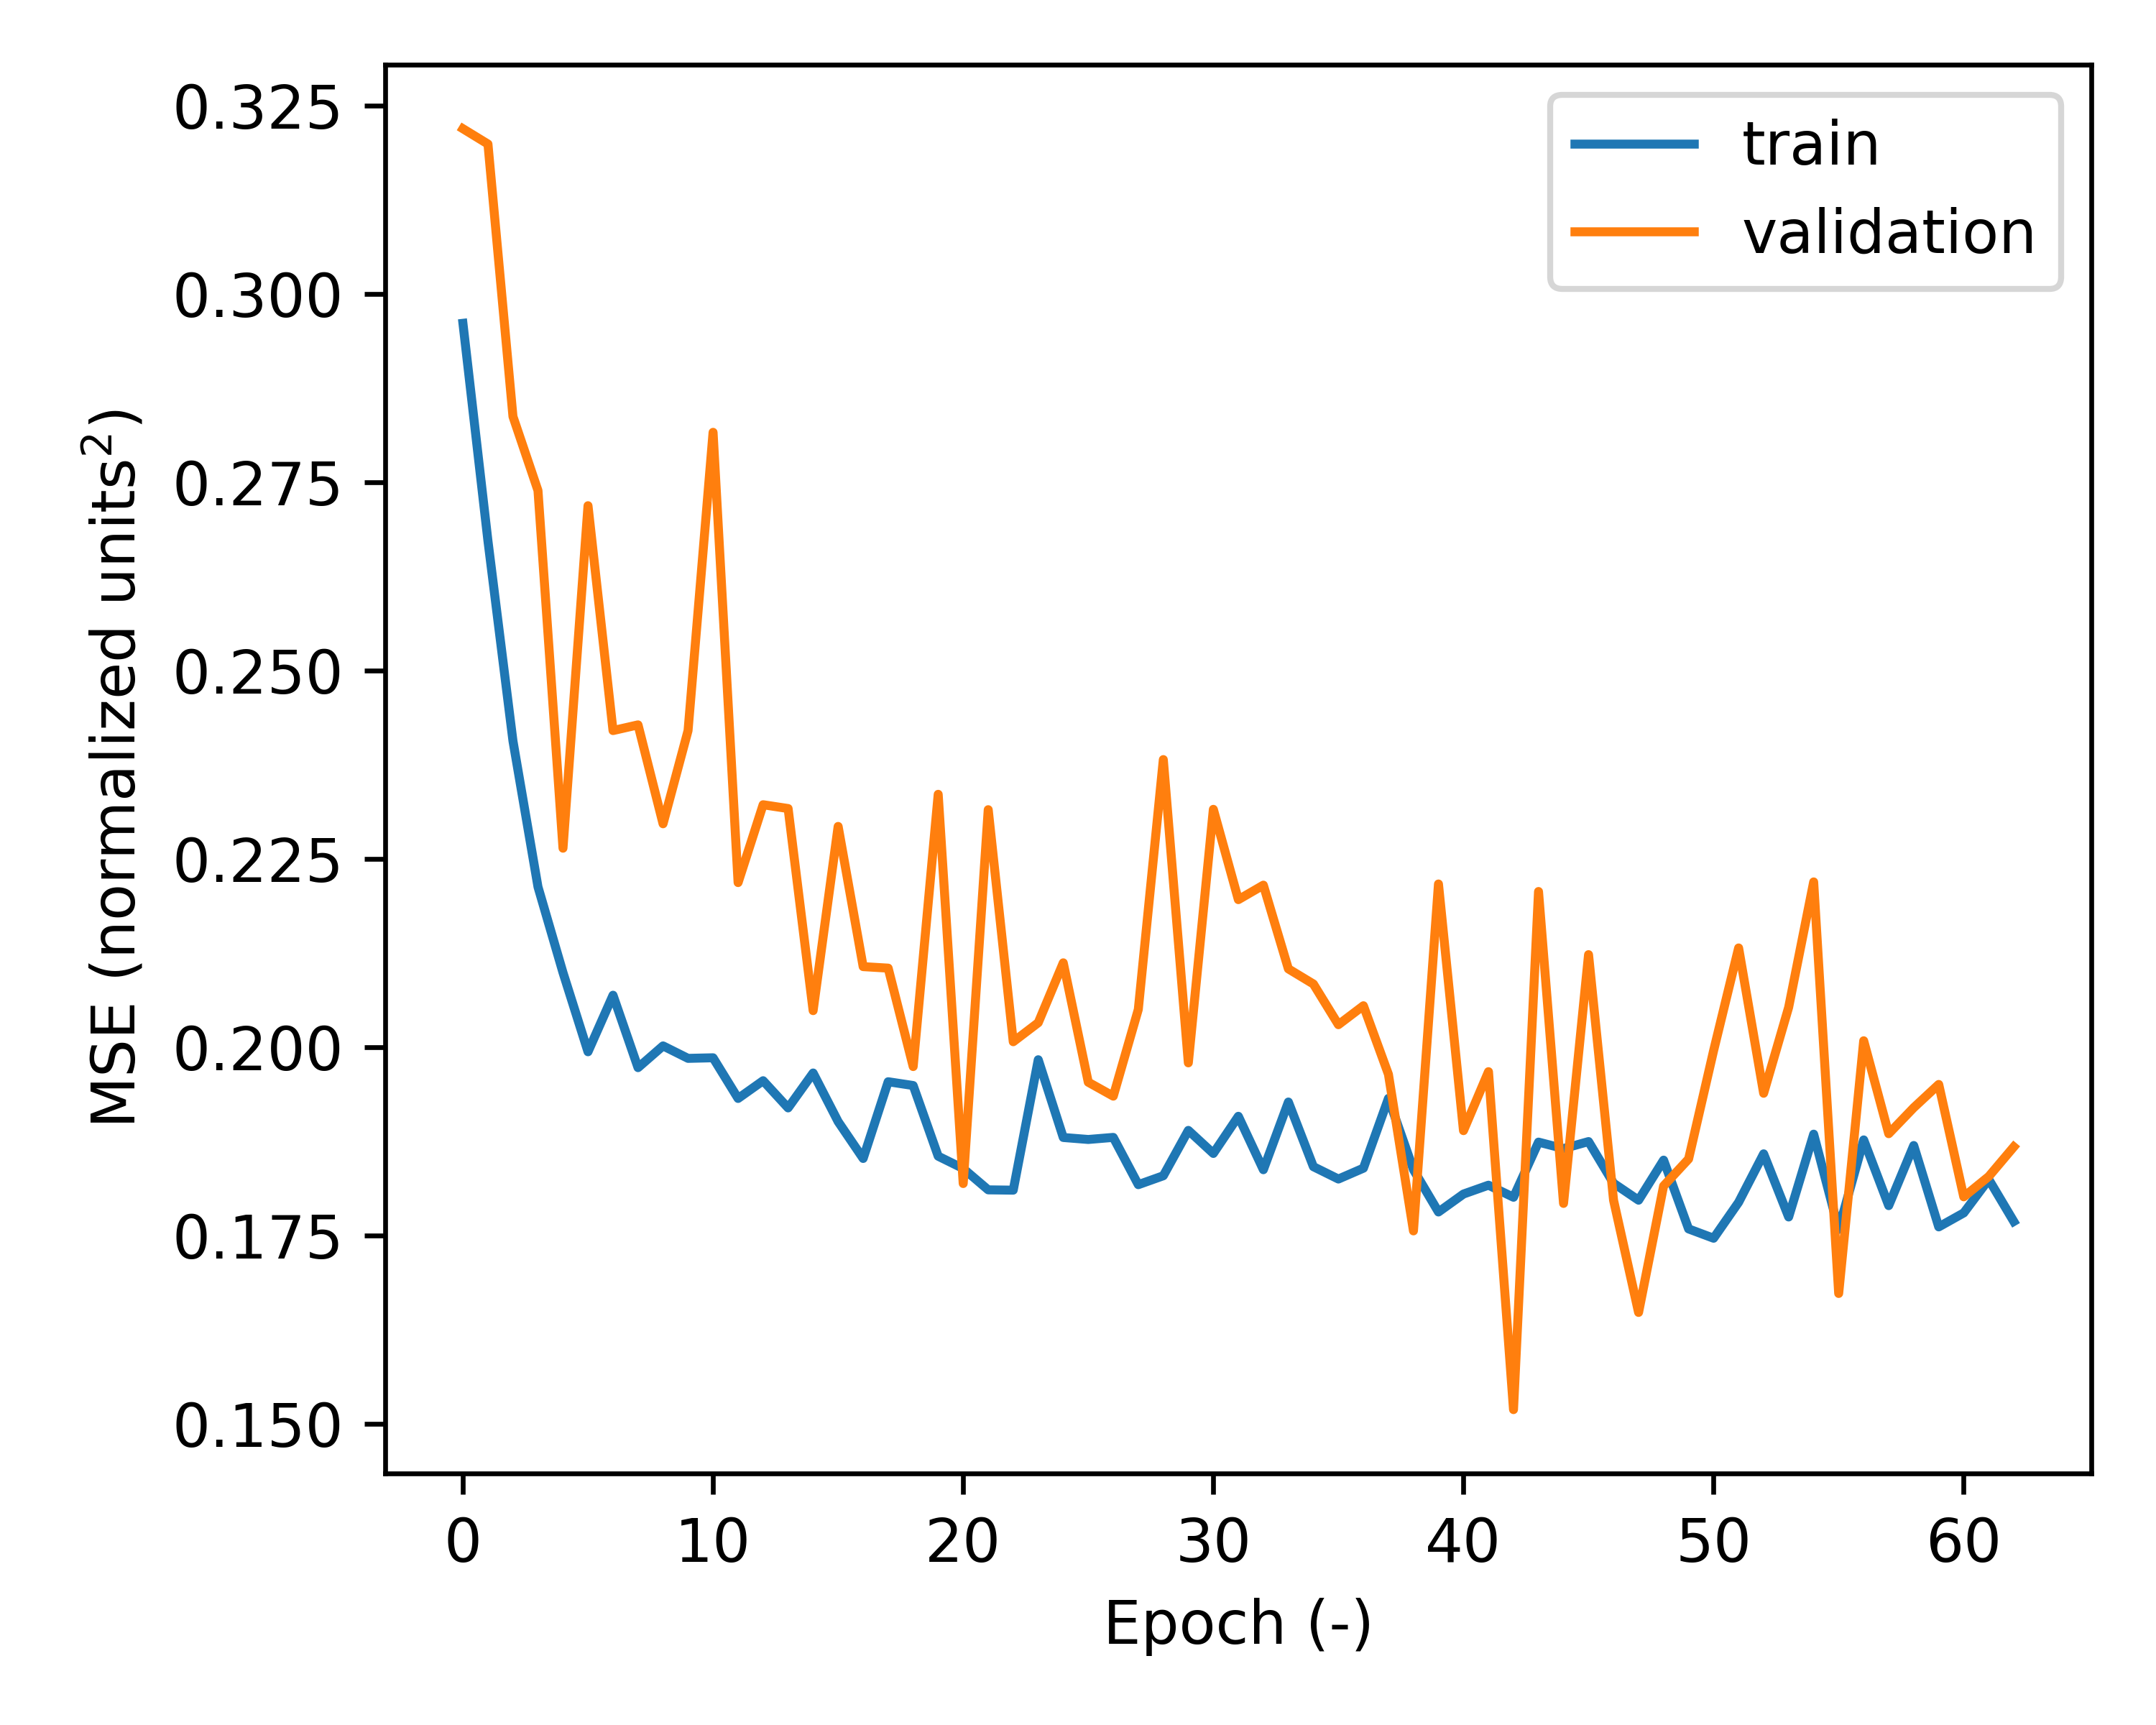
\includegraphics[width=0.46\linewidth]{loss_curve_multi.png}
\caption{Perda de treinamento e validação (MSE) da SNN multimodal selecionada.}
\label{fig:loss_curve_method}
\end{figure}



\FloatBarrier
